% Options for packages loaded elsewhere
\PassOptionsToPackage{unicode}{hyperref}
\PassOptionsToPackage{hyphens}{url}
%
\documentclass[
]{article}
\usepackage{amsmath,amssymb}
\usepackage{lmodern}
\usepackage{iftex}
\ifPDFTeX
  \usepackage[T1]{fontenc}
  \usepackage[utf8]{inputenc}
  \usepackage{textcomp} % provide euro and other symbols
\else % if luatex or xetex
  \usepackage{unicode-math}
  \defaultfontfeatures{Scale=MatchLowercase}
  \defaultfontfeatures[\rmfamily]{Ligatures=TeX,Scale=1}
\fi
% Use upquote if available, for straight quotes in verbatim environments
\IfFileExists{upquote.sty}{\usepackage{upquote}}{}
\IfFileExists{microtype.sty}{% use microtype if available
  \usepackage[]{microtype}
  \UseMicrotypeSet[protrusion]{basicmath} % disable protrusion for tt fonts
}{}
\makeatletter
\@ifundefined{KOMAClassName}{% if non-KOMA class
  \IfFileExists{parskip.sty}{%
    \usepackage{parskip}
  }{% else
    \setlength{\parindent}{0pt}
    \setlength{\parskip}{6pt plus 2pt minus 1pt}}
}{% if KOMA class
  \KOMAoptions{parskip=half}}
\makeatother
\usepackage{xcolor}
\IfFileExists{xurl.sty}{\usepackage{xurl}}{} % add URL line breaks if available
\IfFileExists{bookmark.sty}{\usepackage{bookmark}}{\usepackage{hyperref}}
\hypersetup{
  pdftitle={AT-3},
  pdfauthor={Koushik},
  hidelinks,
  pdfcreator={LaTeX via pandoc}}
\urlstyle{same} % disable monospaced font for URLs
\usepackage[margin=1in]{geometry}
\usepackage{color}
\usepackage{fancyvrb}
\newcommand{\VerbBar}{|}
\newcommand{\VERB}{\Verb[commandchars=\\\{\}]}
\DefineVerbatimEnvironment{Highlighting}{Verbatim}{commandchars=\\\{\}}
% Add ',fontsize=\small' for more characters per line
\usepackage{framed}
\definecolor{shadecolor}{RGB}{248,248,248}
\newenvironment{Shaded}{\begin{snugshade}}{\end{snugshade}}
\newcommand{\AlertTok}[1]{\textcolor[rgb]{0.94,0.16,0.16}{#1}}
\newcommand{\AnnotationTok}[1]{\textcolor[rgb]{0.56,0.35,0.01}{\textbf{\textit{#1}}}}
\newcommand{\AttributeTok}[1]{\textcolor[rgb]{0.77,0.63,0.00}{#1}}
\newcommand{\BaseNTok}[1]{\textcolor[rgb]{0.00,0.00,0.81}{#1}}
\newcommand{\BuiltInTok}[1]{#1}
\newcommand{\CharTok}[1]{\textcolor[rgb]{0.31,0.60,0.02}{#1}}
\newcommand{\CommentTok}[1]{\textcolor[rgb]{0.56,0.35,0.01}{\textit{#1}}}
\newcommand{\CommentVarTok}[1]{\textcolor[rgb]{0.56,0.35,0.01}{\textbf{\textit{#1}}}}
\newcommand{\ConstantTok}[1]{\textcolor[rgb]{0.00,0.00,0.00}{#1}}
\newcommand{\ControlFlowTok}[1]{\textcolor[rgb]{0.13,0.29,0.53}{\textbf{#1}}}
\newcommand{\DataTypeTok}[1]{\textcolor[rgb]{0.13,0.29,0.53}{#1}}
\newcommand{\DecValTok}[1]{\textcolor[rgb]{0.00,0.00,0.81}{#1}}
\newcommand{\DocumentationTok}[1]{\textcolor[rgb]{0.56,0.35,0.01}{\textbf{\textit{#1}}}}
\newcommand{\ErrorTok}[1]{\textcolor[rgb]{0.64,0.00,0.00}{\textbf{#1}}}
\newcommand{\ExtensionTok}[1]{#1}
\newcommand{\FloatTok}[1]{\textcolor[rgb]{0.00,0.00,0.81}{#1}}
\newcommand{\FunctionTok}[1]{\textcolor[rgb]{0.00,0.00,0.00}{#1}}
\newcommand{\ImportTok}[1]{#1}
\newcommand{\InformationTok}[1]{\textcolor[rgb]{0.56,0.35,0.01}{\textbf{\textit{#1}}}}
\newcommand{\KeywordTok}[1]{\textcolor[rgb]{0.13,0.29,0.53}{\textbf{#1}}}
\newcommand{\NormalTok}[1]{#1}
\newcommand{\OperatorTok}[1]{\textcolor[rgb]{0.81,0.36,0.00}{\textbf{#1}}}
\newcommand{\OtherTok}[1]{\textcolor[rgb]{0.56,0.35,0.01}{#1}}
\newcommand{\PreprocessorTok}[1]{\textcolor[rgb]{0.56,0.35,0.01}{\textit{#1}}}
\newcommand{\RegionMarkerTok}[1]{#1}
\newcommand{\SpecialCharTok}[1]{\textcolor[rgb]{0.00,0.00,0.00}{#1}}
\newcommand{\SpecialStringTok}[1]{\textcolor[rgb]{0.31,0.60,0.02}{#1}}
\newcommand{\StringTok}[1]{\textcolor[rgb]{0.31,0.60,0.02}{#1}}
\newcommand{\VariableTok}[1]{\textcolor[rgb]{0.00,0.00,0.00}{#1}}
\newcommand{\VerbatimStringTok}[1]{\textcolor[rgb]{0.31,0.60,0.02}{#1}}
\newcommand{\WarningTok}[1]{\textcolor[rgb]{0.56,0.35,0.01}{\textbf{\textit{#1}}}}
\usepackage{graphicx}
\makeatletter
\def\maxwidth{\ifdim\Gin@nat@width>\linewidth\linewidth\else\Gin@nat@width\fi}
\def\maxheight{\ifdim\Gin@nat@height>\textheight\textheight\else\Gin@nat@height\fi}
\makeatother
% Scale images if necessary, so that they will not overflow the page
% margins by default, and it is still possible to overwrite the defaults
% using explicit options in \includegraphics[width, height, ...]{}
\setkeys{Gin}{width=\maxwidth,height=\maxheight,keepaspectratio}
% Set default figure placement to htbp
\makeatletter
\def\fps@figure{htbp}
\makeatother
\setlength{\emergencystretch}{3em} % prevent overfull lines
\providecommand{\tightlist}{%
  \setlength{\itemsep}{0pt}\setlength{\parskip}{0pt}}
\setcounter{secnumdepth}{-\maxdimen} % remove section numbering
\ifLuaTeX
  \usepackage{selnolig}  % disable illegal ligatures
\fi

\title{AT-3}
\author{Koushik}
\date{2022-05-25}

\begin{document}
\maketitle

\hypertarget{r-markdown}{%
\subsection{R Markdown}\label{r-markdown}}

This is an R Markdown document. Markdown is a simple formatting syntax
for authoring HTML, PDF, and MS Word documents. For more details on
using R Markdown see \url{http://rmarkdown.rstudio.com}.

When you click the \textbf{Knit} button a document will be generated
that includes both content as well as the output of any embedded R code
chunks within the document. You can embed an R code chunk like this:

\begin{Shaded}
\begin{Highlighting}[]
\FunctionTok{summary}\NormalTok{(cars)}
\end{Highlighting}
\end{Shaded}

\begin{verbatim}
##      speed           dist       
##  Min.   : 4.0   Min.   :  2.00  
##  1st Qu.:12.0   1st Qu.: 26.00  
##  Median :15.0   Median : 36.00  
##  Mean   :15.4   Mean   : 42.98  
##  3rd Qu.:19.0   3rd Qu.: 56.00  
##  Max.   :25.0   Max.   :120.00
\end{verbatim}

\hypertarget{including-plots}{%
\subsection{Including Plots}\label{including-plots}}

You can also embed plots, for example:

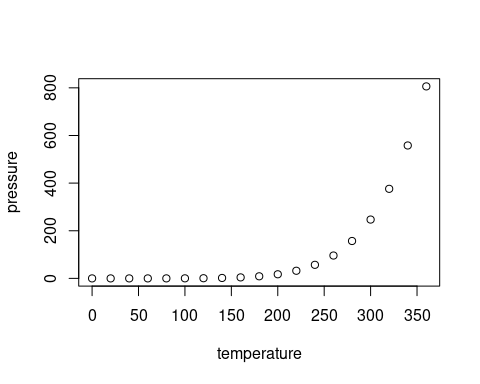
\includegraphics{R-markdown_part_1_files/figure-latex/pressure-1.pdf}

Note that the \texttt{echo\ =\ FALSE} parameter was added to the code
chunk to prevent printing of the R code that generated the plot.

URL=
``\url{https://raw.githubusercontent.com/markziemann/SLE712_files/master/assessment_task3/bioinfo_asst3_part1_files/gene_expression.tsv}''
NAME= ``gene\_expression.tsv'' download.file(URL,destfile=NAME)

URL=
``\url{https://raw.githubusercontent.com/markziemann/SLE712_files/master/assessment_task3/bioinfo_asst3_part1_files/growth_data.csv}''
NAME= ``growth\_data.csv'' download.file(URL,destfile=NAME) \#\#\# HEAD

read.delim(``gene\_expression.tsv'')
head(read.delim(``gene\_expression.tsv''))
str(read.delim(``gene\_expression.tsv''))

cds = read.delim(``gene\_expression.tsv'')

head(cds) row.names(cds) row.names(cds) = cds\$Name\_Description
row.names(cds) \#\#Change the name of the row from a number to the name
of the gene

head(cds,6) \#\#Display the values of the first six data

head(rowMeans(cds{[}2:4{]})) cds\$mean = rowMeans(cds{[}2:4{]})
head(cds,6) \#\#Add a column to show the average of the gene values and
display the first six sets of data

order(-cds\(mean) sorted <- cds[order(-cds\)mean),{]}
sorted{[},c(4,ncol(sorted)){]} head(sorted{[},c(4,ncol(sorted)){]},10)
\#\#List the 10 genes with the highest mean expression

subset(cds,mean \textless{} 10) nrow(subset(cds,mean \textless{} 10))
nrow(cds)

\#\#List the number of rows with gene means less than 10 and calculate
how many rows there are and what the total number of rows is

hist(cds\$mean,xlab=``mean'', main=``Histogram of means'')
*\href{http://ziemann-lab.net:8787/files/project/ast\%203/Histogram.png}{picture}
\#\#\#The following is an analysis of the data `growth\_data.csv'

read.csv(``growth\_data.csv'')

cdss = read.csv(``growth\_data.csv'') head(cdss) colnames(cdss) \#\#Read
the document,and displays the column name

cdss{[}cdss\(Site=="northeast",] site1 = cdss[cdss\)Site==``northeast'',{]}
cdss{[}cdss\(Site=="southwest",] site2 = cdss[cdss\)Site==``southwest'',{]}
mean(site1{[},3{]}) sd(site1{[},3{]}) mean(site1{[},6{]})
sd(site1{[},6{]}) mean(site2{[},3{]}) sd(site2{[},3{]})
mean(site2{[},6{]}) sd(site2{[},6{]}) \#\#site1 is all the data in the
northeast location tree, site2 is the data in the southwest location
tree, determine the data and calculate the standard deviation and mean
respectively

boxplot(site1\(Circumf_2005_cm, site1\)Circumf\_2020\_cm,
ylab=``circumference'', main=``The northeast position starts and ends
with the data'', names = c(``start'',``end''))

boxplot(site2\(Circumf_2005_cm, site2\)Circumf\_2020\_cm,
ylab=``circumference'', main=``The southwest position starts and ends
with the data'', names = c(``start'',``end'')) \#\#The data has already
been sorted in the previous step, so you just need to do the box plot in
this step.

site1gr = mean(site1{[},6{]})-mean(site1{[},4{]})
site1gr/mean(site1{[},4{]})

site2gr = mean(site2{[},6{]})-mean(site2{[},4{]})
site2gr/mean(site2{[},4{]})

\#\#Calculation of the growth rate \#\#step1: The present value is
subtracted from the past value \#\#step2: the result is divided by the
past value

myfunc1 = function(x,y)\{ t.test(x,y)

rest = t.test(x,y) PVAL = rest\$p.value boxplot(x,y)
HEADER=paste(``P:'',PVAL) mtext(HEADER) \}

t.test(cdss\(Circumf_2020_cm - cdss\)Circumf\_2010\_cm\textasciitilde cdss\(Site) boxplot(cdss\)Circumf\_2020\_cm
- cdss\(Circumf_2010_cm~cdss\)Site,xlab = ``location'',ylab =
``growth'') PVAL =
t.test(cdss\(Circumf_2020_cm - cdss\)Circumf\_2010\_cm\textasciitilde cdss\(Site)\)p.value
HEADER=paste(``P:'',PVAL) mtext(HEADER)

wilcox.test(cdss\(Circumf_2020_cm - cdss\)Circumf\_2010\_cm\textasciitilde cdss\(Site) boxplot(cdss\)Circumf\_2020\_cm
- cdss\(Circumf_2010_cm~cdss\)Site,xlab = ``location'',ylab =
``growth'') PVAL =
wilcox.test(cdss\(Circumf_2020_cm - cdss\)Circumf\_2010\_cm\textasciitilde cdss\(Site)\)p.value
HEADER=paste(``P:'',PVAL) mtext(HEADER)

\#\#The p-values are calculated using ttest and wilcox.test
respectively, and it can be seen that the p-values calculated using
ttest are smaller, and the differences in the data over 10 years are
directly applied in the calculation, and no mean values are involved

\end{document}
